\documentclass{amsart}
\synctex=1

%=================================================================
% 
\newcount\DraftStatus  % 0 suppresses notes to selves in text
\DraftStatus=1   % TODO: set to 0 for final version
%=================================================================

%=================================================================
\usepackage{comment}
%=================================================================
%
\includecomment{JournalOnly}  
\includecomment{ConferenceOnly}  
\includecomment{TulipStyle}
%
%=================================================================
\input{preamble}


%=================================================================
%
\begin{document}
%
%=================================================================
%
\title[Lin's Flip0103]{Flip0103 Final Presetantion Report}%

\author{Shuxia Lin}
\address[A.~1]{School of Computer Science,\\ 
SouthEast University, NanJing 211189, China}%
\email[A.~1]{shuxia.lin@tulip.org.au}


%\thanks{Thanks to \ldots}%
\subjclass{Artificial Intelligence}%
\keywords{Machine Learning, Data Mining, ...}%
\date{\gitAuthorDate}%

\begin{abstract}

While research on emotions has become 
one of the most productive areas at 
the intersection of cognitive science, 
artificial intelligence and natural language processing,
the diversity and incommensurability of 
emotion models seriously hampers progress in the field.
Models of emotion are commonly divided into
categorical and dimensional ones.
Compared to the categorical approach
that represents affective states as 
several discrete classes (e.g., positive and negative),
the dimensional approach represents
affective states as continuous numerical values 
on multiple dimensions,
such as the valence-arousal-dominance (VAD) space,
thus allowing for 
more fine-grained sentiment analysis. 
In building dimensional sentiment applications, 
affective lexicons
with valence-arousal-dominance ratings are 
useful resources but 
are still very rare.
In this paper, 
we propose a novel approach
based on emotion distribution learning.
The key idea is to learn a mapping function
from sentences to their dimensional emotion distributions
by the proposed 
Dimensional Emotion Distribution Learning(DEDL)
method.
And then,
we use the predicted value of VAD and 
the notational VAD to 
classification the emotion category.

\end{abstract}

\maketitle
\tableofcontents

\newpage
%=================================================================

%=================================================================
\section{Introduction}\label{sec-intro}


Emotion detection has attracted great interest 
in the natural language processing (NLP)
in the last few years.
In sentiment analysis, 
affective states are generally represented 
using either categorical or dimensional approaches.
The most popular categorical approach represents is 
Ekman’s six basic emotions 
(e.g., anger, happiness, fear, sadness, disgust and surprise)
The dimensional approach represents affective states by using
continuous numerical values in two/three dimensions,.
The valence-arousal (VA) dimensions model , 
as shown in ~\Cref{fig:va} . 
The valence represents the degree of 
positive and negative, 
while the arousal represents the degree of 
excitement and calm. 
In 1994,
Bradley and Lang proposed 
Valence- Arousal-Dominance model,
as shown in ~\Cref{fig:vad}.
And Dominance perceived degree of control in a (social) situation.
Based on this representation, 
any affective state can be represented as a point 
in the VA/VAD coordinate plane. 

In this paper, 
we want to predict  
multiple emotion dimension scores for an input text.
A new machine learning paradigm called 
Label Distribution Learning (LDL) 
was proposed in recently years.
Similarly,
we propose an dimensional emotion distribution learning (DEDL) algorithm
Different from the previous approaches, 
DEDL assumes that
each sentence contains a mixture of 
dimensional emotions with different intensities. 
We can label each sentence with 
an label distribution vector 
where elements corresponds to 
dimensional emotions and 
the value of each element indicates the intensity of the dimensional emotions. 
We require that each vector element has a value 
between 0 and 1 and they sum up to 1.

\begin{figure}[htbp]
	\begin{minipage}[t]{0.5\linewidth}
		\centering
		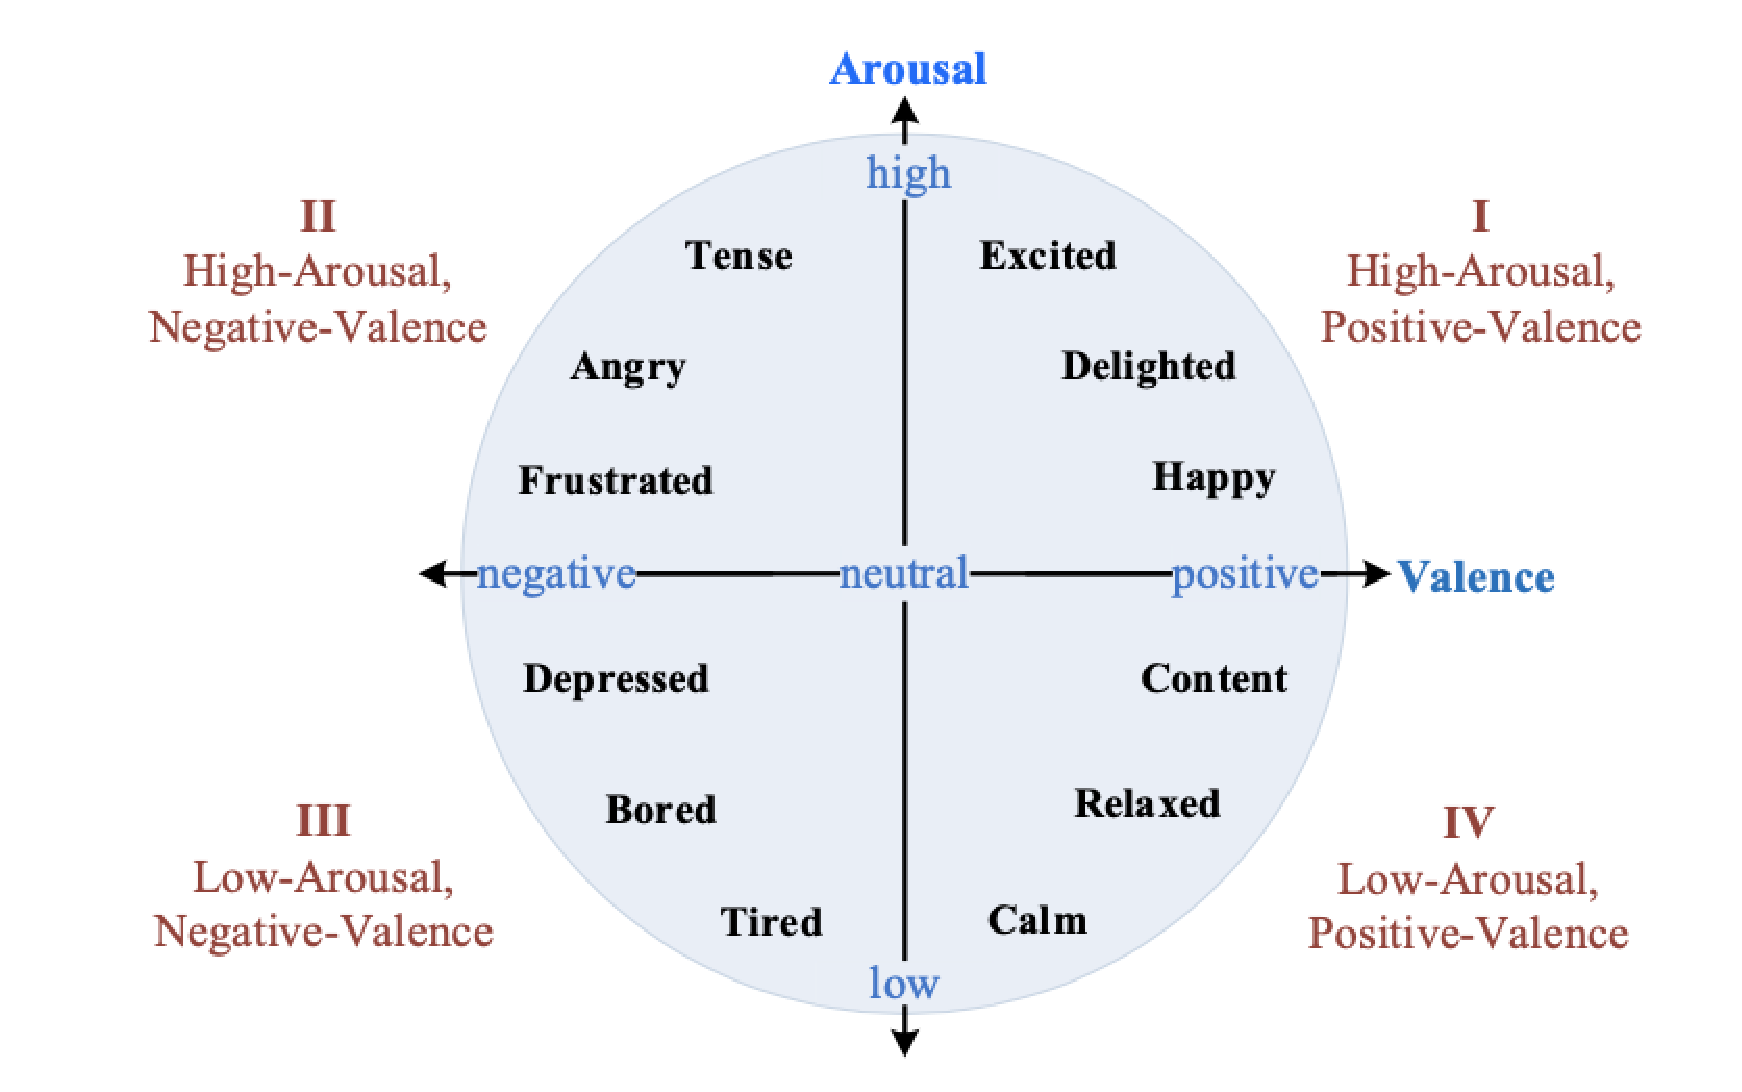
\includegraphics[height=4cm,width=6cm]{figures/va_emotion.eps}
		\caption{The emotional space spanned by the Valence-Arousal model}\label{fig:va}
	\end{minipage}%
	\hfill
	\begin{minipage}[t]{0.5\linewidth}
		\centering
		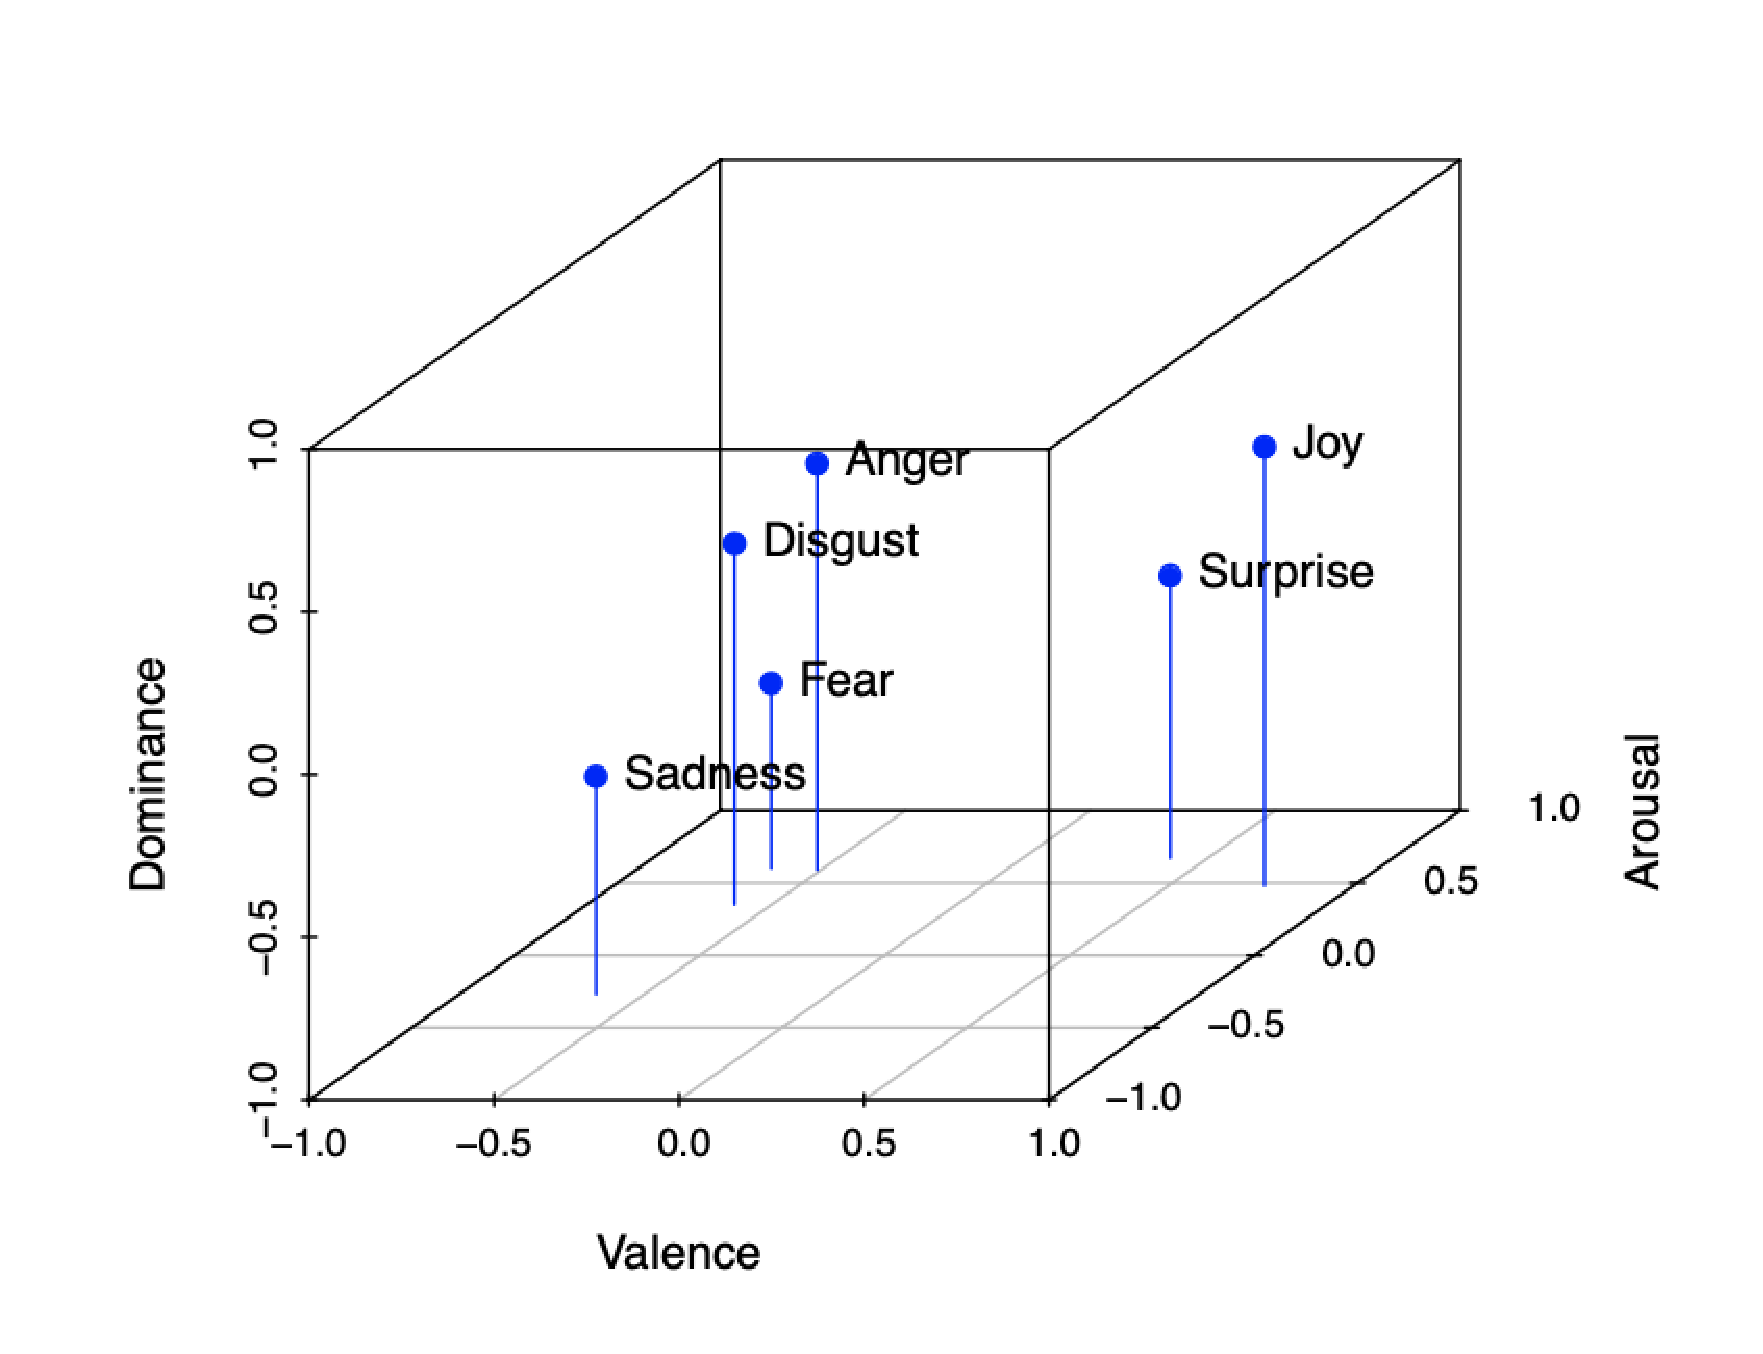
\includegraphics[height=4cm,width=6cm]{figures/six_emotions_vad.eps}
		\caption{The emotional space spanned by the Valence-Arousal-Dominance model. }\label{fig:vad}
	\end{minipage}
\end{figure}

%%Based on this representation, any affective state can be represented as a point in the VA coordinate plane. 



\begin{equation}\label{eq:test}
a = b \times \sqrt{ab}
\end{equation}


\section{Preliminaries} \label{sec-preliminaries}

\blindtext

\gliMarker  %TODO: GLi Here


\section{Method} \label{sec-method}

\blindtext
\blindlist{itemize}[3]
\blinditemize
\blindenumerate

\blindmathtrue
\blindmathfalse
\blinddescription

\sxlinMarker %TODO: QWu Here

\section{Experiment and Analysis} \label{sec-experiment}


\begin{table}  \centering
  \caption{Precision Comparison on Event Detection Methods}
  \label{tbl:overall-experiments}
  \begin{tabular}{cccc}
\toprule
    % after \\: \hline or \cline{col1-col2} \cline{col3-col4} ...
    & OR Event Detection & AC Event Detection & TC Event Detection \\
\midrule
    precision & 0.83 & 0.69 & 0.46 \\
    recall & 0.68 & 0.48 & 0.36 \\
    F-score & 0.747 & 0.57 & 0.4 \\
\bottomrule
\end{tabular}
\end{table}


\section{Conclusions} \label{sec-conclusions}

\blindtext

\section*{Acknowledgment}

\lipsum[1]


The authors would like to thank \ldots



% ----------------------------------------------------------------
\newpage
\bibliography{tuliplab,yourbib}
\bibliographystyle{plainnat}
%=================================================================

%\listoftodos

\end{document}

